\documentclass[multi=page, border=0.5cm]{standalone}
\usepackage{calculator}
\usepackage[svgnames]{xcolor}
\usepackage{tikz}

\tikzset{
    poly/.style={ line width=1mm, red },
    edge/.style={ line width=0.5mm, red },
    vertex/.style={ shape=coordinate },
    shadow1/.style={ black, opacity=0.15, fill },
    shadow2/.style={ black, opacity=0.25, fill }
}


\definecolor{light-gray}{gray}{0.95}

\begin{document}
\begin{page}
    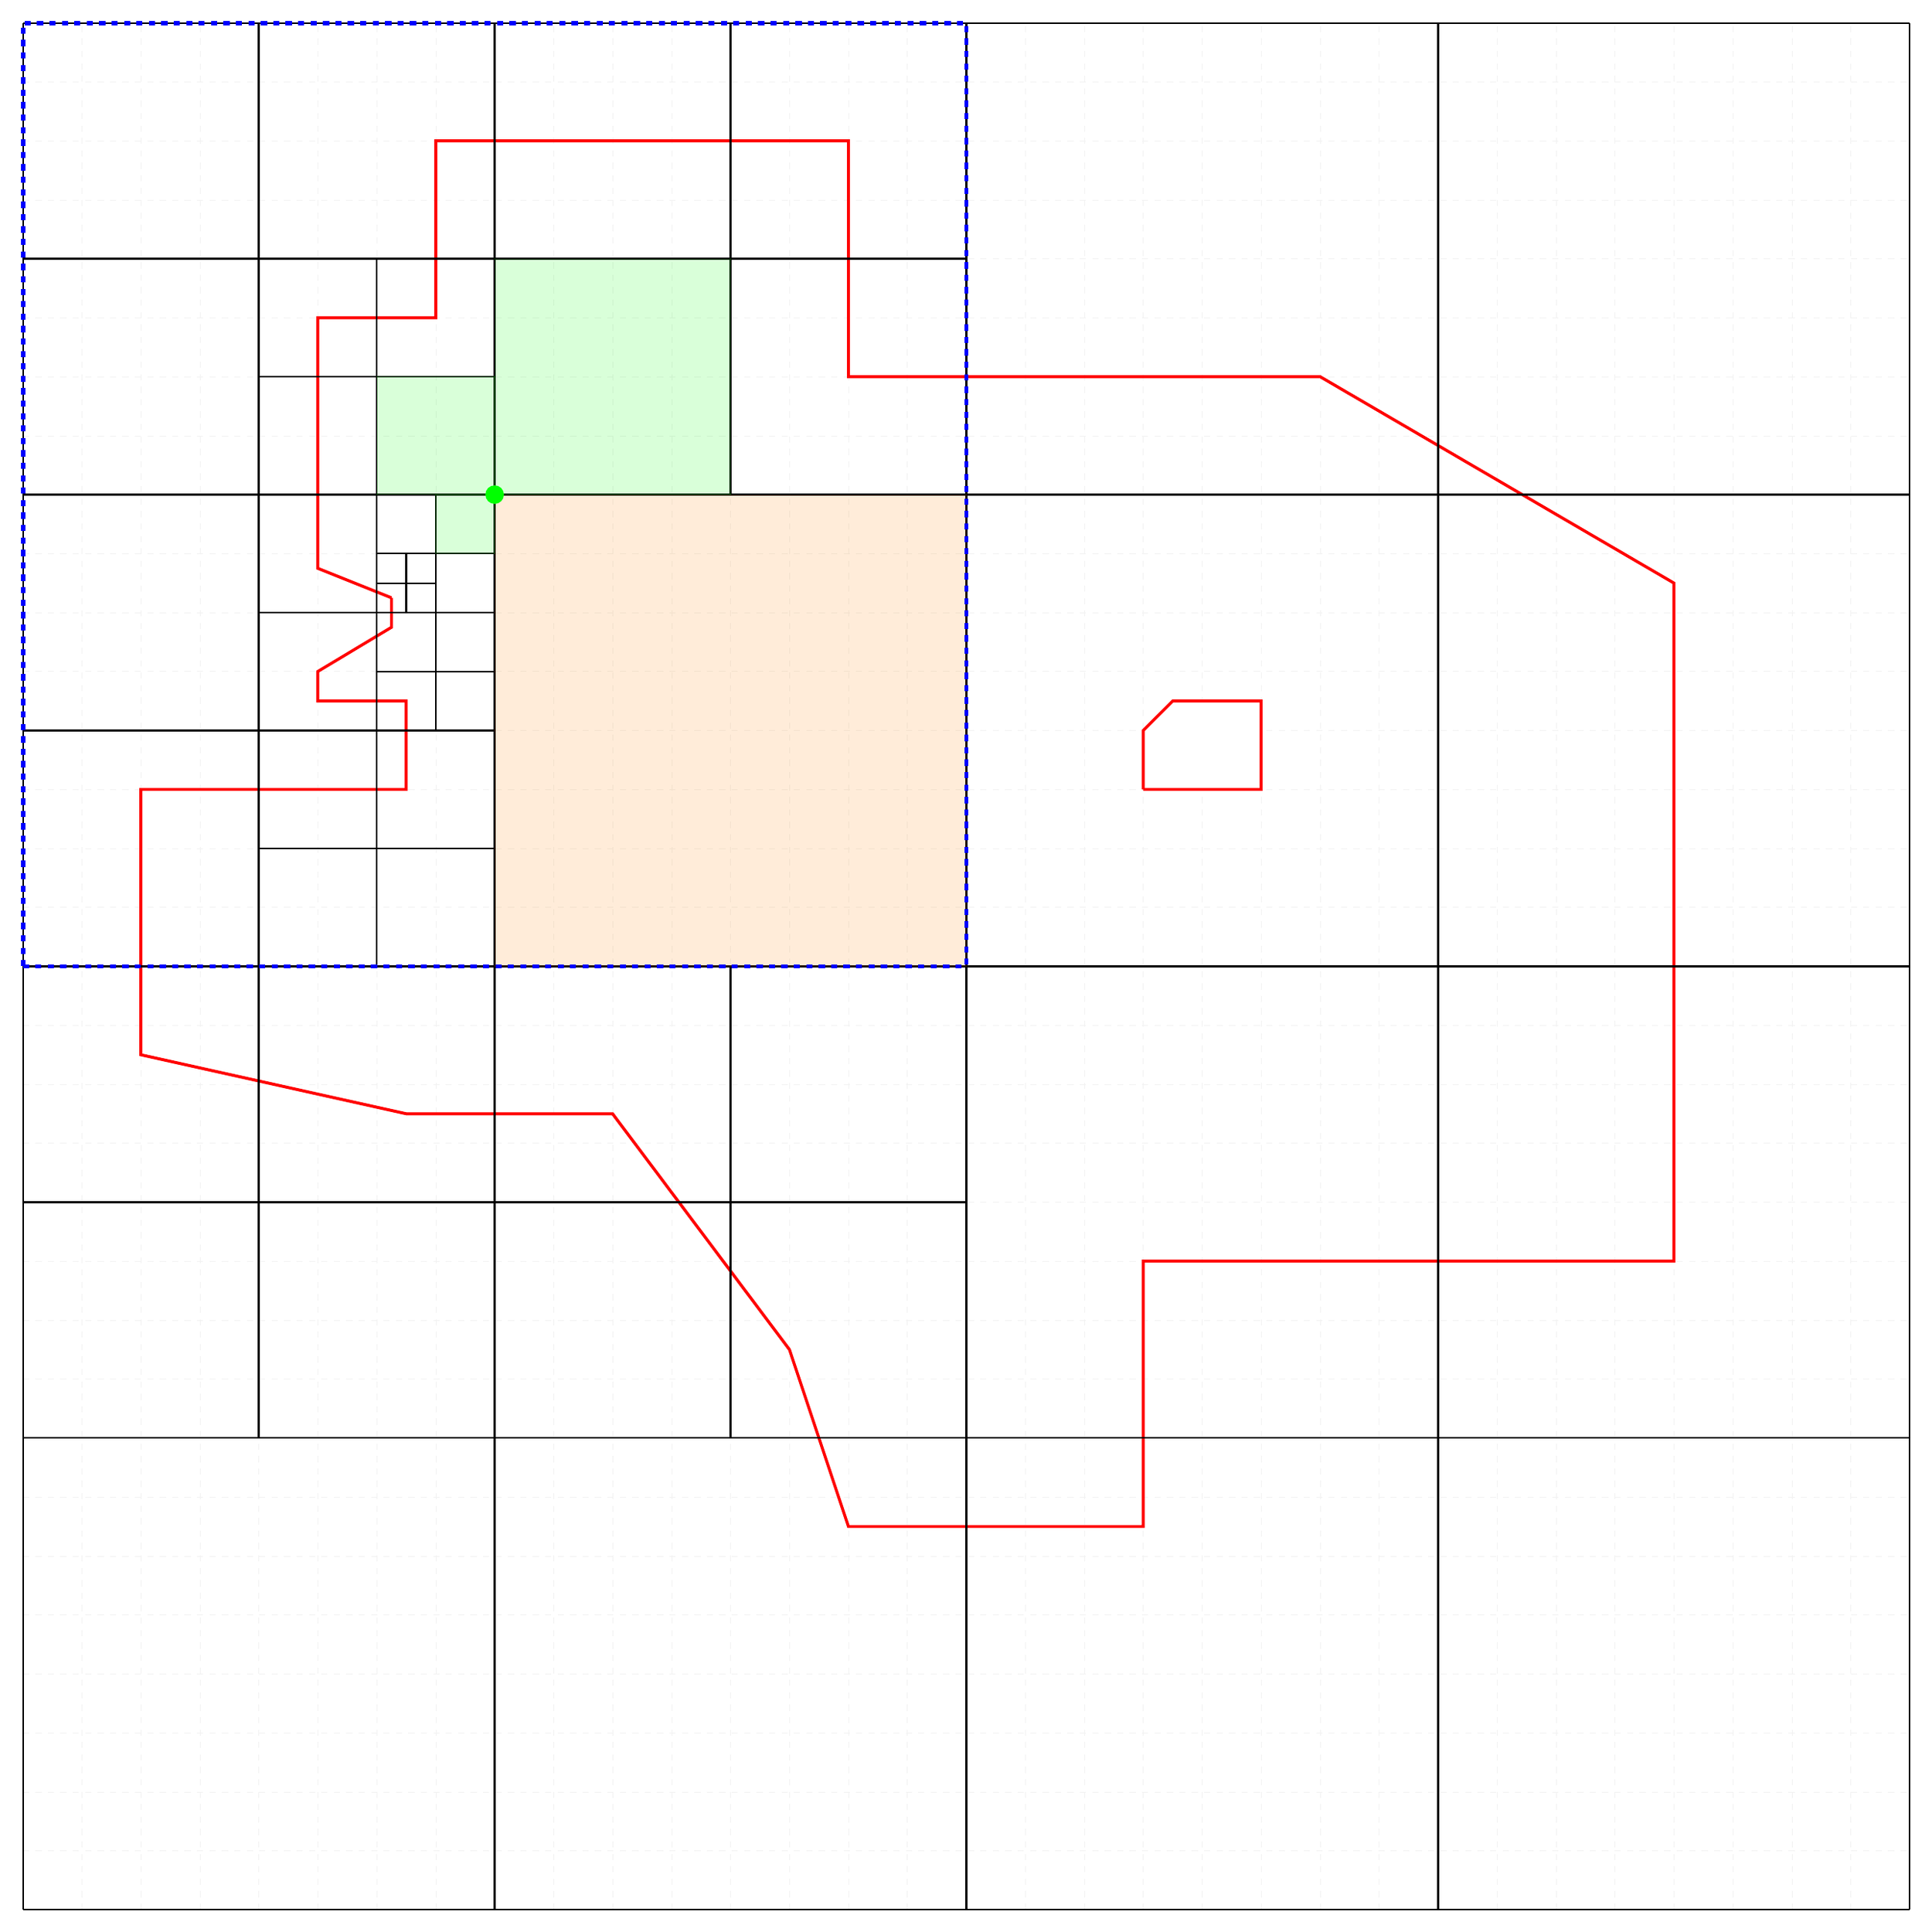
\begin{tikzpicture}
        \draw[step=1, very thin, light-gray, dashed] (0,0) grid (32,32);

        \coordinate (a1) at (6.25, 22.25); \coordinate (a2) at (5, 21);
        \coordinate (a3) at (5, 20.5); \coordinate (a4) at (6.5, 20.5);
        \coordinate (a5) at (6.5, 19); \coordinate (a6) at (2, 19);
        \coordinate (a7) at (2, 14.5); \coordinate (a8) at (6.5, 13.5);
        \coordinate (a9) at (10, 13.5); \coordinate (a10) at (13, 9.5);
        \coordinate (a11) at (14, 9.5); \coordinate (a11) at (14, 6.5);
        \coordinate (a12) at (19, 6.5); \coordinate (a13) at (19, 11);
        \coordinate (a14) at (28, 11); \coordinate (a15) at (28, 22.5);
        \coordinate (a16) at (22, 26); \coordinate (a17) at (14, 26);
        \coordinate (a18) at (14, 30); \coordinate (a19) at (7, 30);
        \coordinate (a20) at (7, 27); \coordinate (a21) at (5, 27);
        \coordinate (a22) at (5, 22.75);
        \coordinate (b) at (6.25, 21.75);

        \draw[edge] (a1) -- (b) -- (a2) -- (a3) -- (a4) -- (a5) -- (a6) -- (a7) -- (a8) -- (a9) -- (a10) -- (a11) -- (a12) -- (a13) -- (a14) -- (a15) -- (a16)
-- (a17) -- (a18) -- (a19) -- (a20) -- (a21) -- (a22) -- (a1);

        \draw[step=8,  thick, black] (0,0)  grid (32,32);
        \draw[step=4,  thick, black] (0,24) grid (8,32);
        \draw[step=4,  thick, black] (0,16) grid (8,24);
        \draw[step=4,  thick, black] (0,8)  grid (8,16);
        \draw[step=4,  thick, black] (8,8)  grid (16,16);
        \draw[step=4,  thick, black] (8,24) grid (16,32);
        \draw[step=2,  thick, black] (4,16) grid (8,20);
        \draw[step=2,  thick, black] (4,20) grid (8,24);
        \draw[step=2,  thick, black] (4,24) grid (8,28);
        \draw[step=1,  thick, black] (6,20) grid (8,24);
        \draw[step=0.5,thick, black] (6,22) grid (7,23);

        \draw[orange, opacity=0.15, fill] (8,16) rectangle (16,24);
        
        \draw[blue, line width=0.75mm, dashed] (0,16) rectangle (16,32);
        
        \draw[green, fill] (8,24) circle (0.15);
        
        \draw[green, opacity=0.15, fill] (7,23) rectangle (8,24);
        \draw[green, opacity=0.15, fill] (6,24) rectangle (8,26);
        \draw[green, opacity=0.15, fill] (8,24) rectangle (12,28);

        \coordinate (h1) at (19, 19); \coordinate (h2) at (21,19);
        \coordinate (h3) at (21, 20.5); \coordinate (h4) at (19.5,20.5);
        \coordinate (h5) at (19, 20); \coordinate (h6) at (19.5,20.5);
        \draw[edge, fill=white] (h1) -- (h2) -- (h3) -- (h4) -- (h5) -- (h1);

    \end{tikzpicture}
\end{page}

\begin{page}
    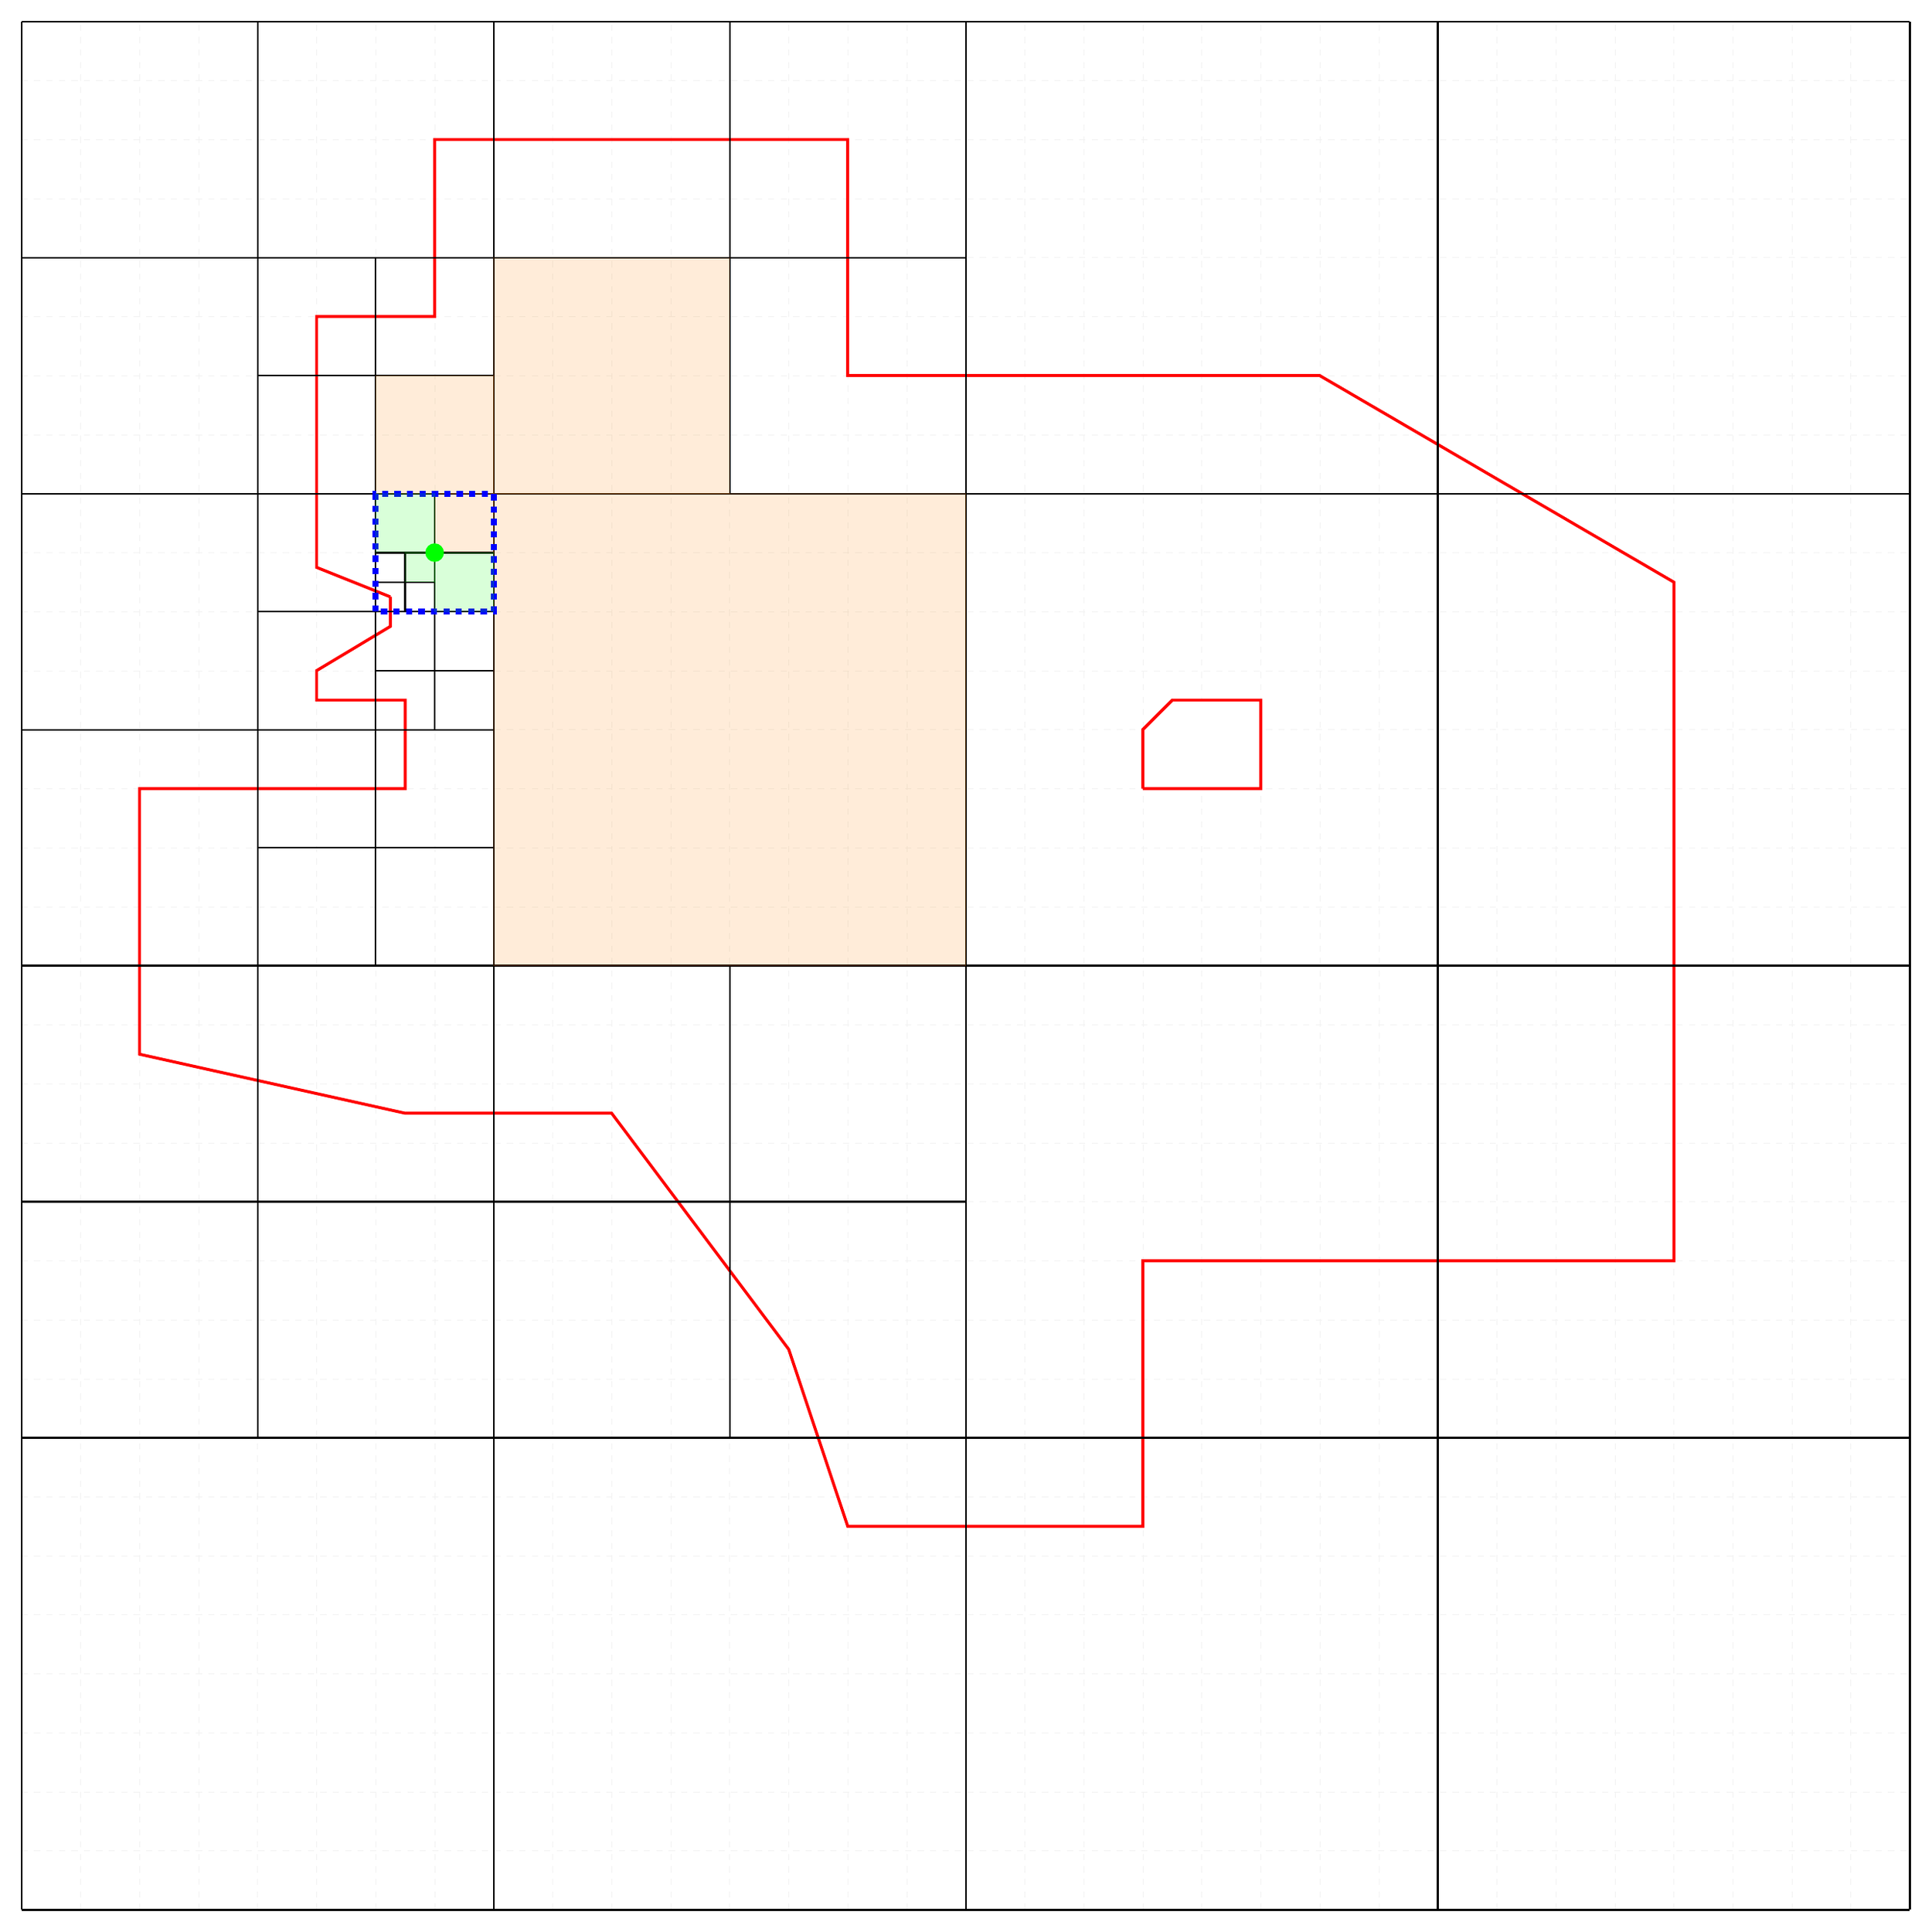
\begin{tikzpicture}
        \draw[step=1, very thin, light-gray, dashed] (0,0) grid (32,32);

        \coordinate (a1) at (6.25, 22.25); \coordinate (a2) at (5, 21);
        \coordinate (a3) at (5, 20.5); \coordinate (a4) at (6.5, 20.5);
        \coordinate (a5) at (6.5, 19); \coordinate (a6) at (2, 19);
        \coordinate (a7) at (2, 14.5); \coordinate (a8) at (6.5, 13.5);
        \coordinate (a9) at (10, 13.5); \coordinate (a10) at (13, 9.5);
        \coordinate (a11) at (14, 9.5); \coordinate (a11) at (14, 6.5);
        \coordinate (a12) at (19, 6.5); \coordinate (a13) at (19, 11);
        \coordinate (a14) at (28, 11); \coordinate (a15) at (28, 22.5);
        \coordinate (a16) at (22, 26); \coordinate (a17) at (14, 26);
        \coordinate (a18) at (14, 30); \coordinate (a19) at (7, 30);
        \coordinate (a20) at (7, 27); \coordinate (a21) at (5, 27);
        \coordinate (a22) at (5, 22.75);
        \coordinate (b) at (6.25, 21.75);

        \draw[edge] (a1) -- (b) -- (a2) -- (a3) -- (a4) -- (a5) -- (a6) -- (a7) -- (a8) -- (a9) -- (a10) -- (a11) -- (a12) -- (a13) -- (a14) -- (a15) -- (a16)
-- (a17) -- (a18) -- (a19) -- (a20) -- (a21) -- (a22) -- (a1);

        \draw[step=8,  thick, black] (0,0)  grid (32,32);
        \draw[step=4,  thick, black] (0,24) grid (8,32);
        \draw[step=4,  thick, black] (0,16) grid (8,24);
        \draw[step=4,  thick, black] (0,8)  grid (8,16);
        \draw[step=4,  thick, black] (8,8)  grid (16,16);
        \draw[step=4,  thick, black] (8,24) grid (16,32);
        \draw[step=2,  thick, black] (4,16) grid (8,20);
        \draw[step=2,  thick, black] (4,20) grid (8,24);
        \draw[step=2,  thick, black] (4,24) grid (8,28);
        \draw[step=1,  thick, black] (6,20) grid (8,24);
        \draw[step=0.5,thick, black] (6,22) grid (7,23);

        \draw[orange, opacity=0.15, fill] (8,16) rectangle (16,24);
        \draw[orange, opacity=0.15, fill] (6,24) rectangle (8,26);
        \draw[orange, opacity=0.15, fill] (8,24) rectangle (12,28);
        \draw[orange, opacity=0.15, fill] (7,23) rectangle (8,24);
        
        \draw[blue, line width=1mm, dashed] (6,22) rectangle (8,24);
        
        \draw[green, opacity=0.15, fill] (6.5,22.5) rectangle (7,23);
        \draw[green, opacity=0.15, fill] (7,22) rectangle (8,23);
        \draw[green, opacity=0.15, fill] (6,23) rectangle (7,24);

        \draw[green, fill] (7,23) circle (0.15);

        \coordinate (h1) at (19, 19); \coordinate (h2) at (21,19);
        \coordinate (h3) at (21, 20.5); \coordinate (h4) at (19.5,20.5);
        \coordinate (h5) at (19, 20); \coordinate (h6) at (19.5,20.5);
        \draw[edge, fill=white] (h1) -- (h2) -- (h3) -- (h4) -- (h5) -- (h1);

    \end{tikzpicture}
\end{page}

\begin{page}
    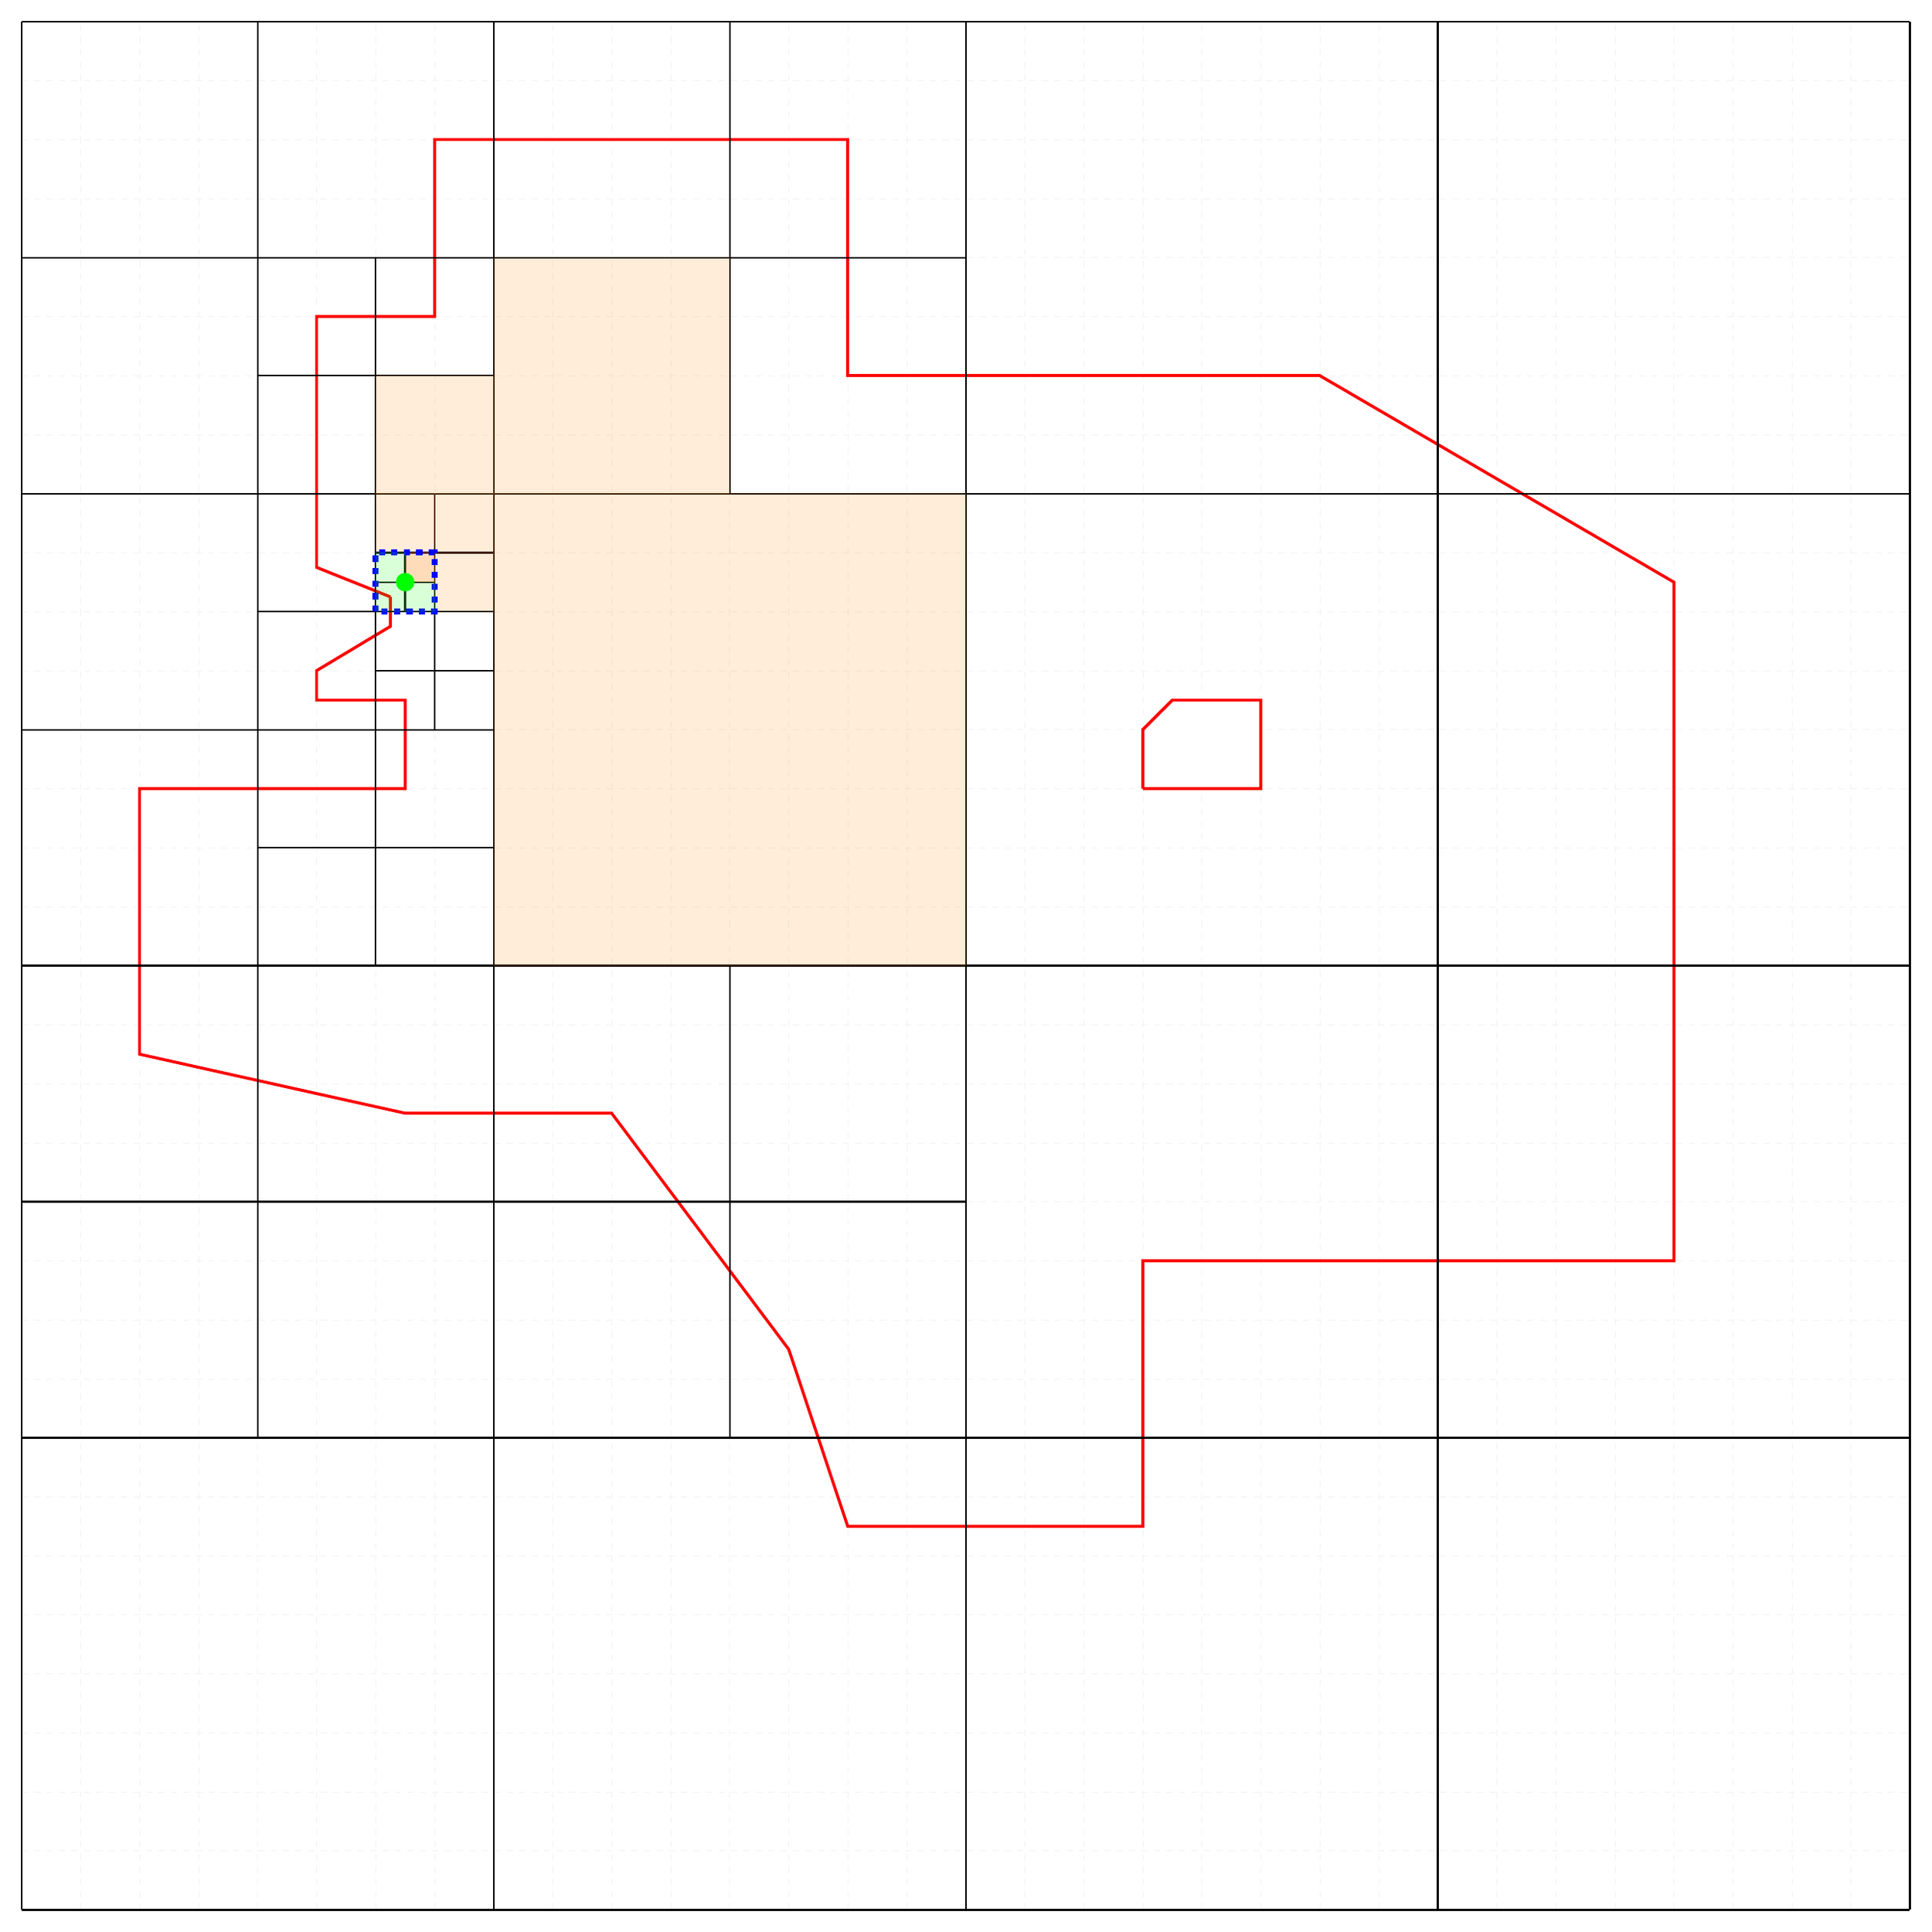
\begin{tikzpicture}
        \draw[step=1, very thin, light-gray, dashed] (0,0) grid (32,32);

        \coordinate (a1) at (6.25, 22.25); \coordinate (a2) at (5, 21);
        \coordinate (a3) at (5, 20.5); \coordinate (a4) at (6.5, 20.5);
        \coordinate (a5) at (6.5, 19); \coordinate (a6) at (2, 19);
        \coordinate (a7) at (2, 14.5); \coordinate (a8) at (6.5, 13.5);
        \coordinate (a9) at (10, 13.5); \coordinate (a10) at (13, 9.5);
        \coordinate (a11) at (14, 9.5); \coordinate (a11) at (14, 6.5);
        \coordinate (a12) at (19, 6.5); \coordinate (a13) at (19, 11);
        \coordinate (a14) at (28, 11); \coordinate (a15) at (28, 22.5);
        \coordinate (a16) at (22, 26); \coordinate (a17) at (14, 26);
        \coordinate (a18) at (14, 30); \coordinate (a19) at (7, 30);
        \coordinate (a20) at (7, 27); \coordinate (a21) at (5, 27);
        \coordinate (a22) at (5, 22.75);
        \coordinate (b) at (6.25, 21.75);

        \draw[edge] (a1) -- (b) -- (a2) -- (a3) -- (a4) -- (a5) -- (a6) -- (a7) -- (a8) -- (a9) -- (a10) -- (a11) -- (a12) -- (a13) -- (a14) -- (a15) -- (a16)
-- (a17) -- (a18) -- (a19) -- (a20) -- (a21) -- (a22) -- (a1);

        \draw[step=8,  thick, black] (0,0)  grid (32,32);
        \draw[step=4,  thick, black] (0,24) grid (8,32);
        \draw[step=4,  thick, black] (0,16) grid (8,24);
        \draw[step=4,  thick, black] (0,8)  grid (8,16);
        \draw[step=4,  thick, black] (8,8)  grid (16,16);
        \draw[step=4,  thick, black] (8,24) grid (16,32);
        \draw[step=2,  thick, black] (4,16) grid (8,20);
        \draw[step=2,  thick, black] (4,20) grid (8,24);
        \draw[step=2,  thick, black] (4,24) grid (8,28);
        \draw[step=1,  thick, black] (6,20) grid (8,24);
        \draw[step=0.5,thick, black] (6,22) grid (7,23);

        \draw[orange, opacity=0.15, fill] (8,16) rectangle (16,24);
        \draw[orange, opacity=0.15, fill] (6,24) rectangle (8,26);
        \draw[orange, opacity=0.15, fill] (8,24) rectangle (12,28);
        \draw[orange, opacity=0.15, fill] (7,23) rectangle (8,24);
        \draw[orange, opacity=0.15, fill] (6.5,22.5) rectangle (7,23);
        \draw[orange, opacity=0.15, fill] (7,22) rectangle (8,23);
        \draw[orange, opacity=0.15, fill] (6,23) rectangle (7,24);
        \draw[orange, opacity=0.15, fill] (6.5,22.5) rectangle (7,23);
        
        \draw[blue, line width=1mm, dashed] (6,22) rectangle (7,23);
        
        \draw[green, opacity=0.15, fill] (6,22)   rectangle (6.5,22.5);
        \draw[green, opacity=0.15, fill] (6,22.5) rectangle (6.5,23);
        \draw[green, opacity=0.15, fill] (6.5,22) rectangle (7,22.5);

        \draw[green, fill] (6.5,22.5) circle (0.15);

        \coordinate (h1) at (19, 19); \coordinate (h2) at (21,19);
        \coordinate (h3) at (21, 20.5); \coordinate (h4) at (19.5,20.5);
        \coordinate (h5) at (19, 20); \coordinate (h6) at (19.5,20.5);
        \draw[edge, fill=white] (h1) -- (h2) -- (h3) -- (h4) -- (h5) -- (h1);

    \end{tikzpicture}
\end{page}
\end{document} 
